\documentclass[10pt,letterpaper,oneside]{article}
\usepackage[letterpaper,margin=0.5in]{geometry}
\usepackage{wrapfig}
\usepackage{mathtools}
\usepackage{amsmath}
\usepackage{mathrsfs}
\usepackage{graphicx}
%\usepackage{luatex}
\usepackage{caption}
\usepackage{subcaption}
\usepackage{tikz-feynman}
\tikzfeynmanset{compat=1.1.0}
\usepackage{feynmp}
\begin{document}
\part{LeptoQuark Mediated Neutrino Mass:}
\section{2$\times$LQ}
2 options: \begin{enumerate}
\item $e_R = + (S) \implies$ tree level
\item $e_R = - (S) \implies$ 1 loop level
\end{enumerate}
\Large
\begin{center}
$m_{\nu}\propto x \left(M_d\right) x\prime$ \quad
$m_{e}\propto x \left(M_u\right) x\prime \prime$ \quad
$h \implies e^- e^+ \left(1+?\right)$ where $\mathcal{A}\sim m_e$ \\
\end{center}
\normalsize
\begin{itemize}
\item Phenomenology of the LQ$\rightarrow$? and h$\rightarrow$? decays?!
\item Rare processes!
\end{itemize} 
\begin{figure}[h]
\centering
\begin{subfigure}[b]{0.4\textwidth}
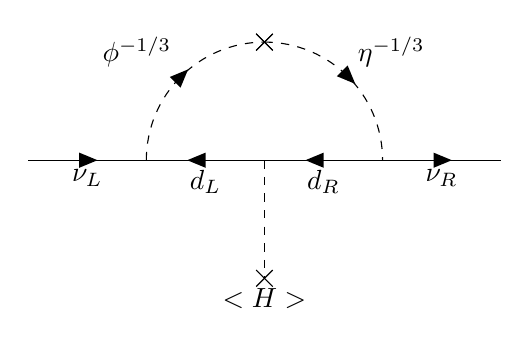
\begin{tikzpicture}
\begin{feynman}
\vertex (i);
\vertex [right = of i] (a);
\vertex [right = of a] (b);
\vertex [right = of b] (c);
\vertex [right = of c] (f);
\vertex [below = of b] (d) {$<H>$};
\vertex [above = of b] (u);
\diagram*{
(i) -- [fermion, edge label' = $\nu_L$] (a) -- [anti fermion, edge label' = $d_L$] (b),
(b) -- [anti fermion, edge label' = $d_R$] (c) -- [fermion, edge label' = $\nu_R$] (f),
(b) -- [scalar, insertion = 1] (d),
(a) -- [charged scalar, quarter left, edge label = $\phi^{-1/3}$] (u)[cross],
(u) -- [charged scalar, insertion = 0, quarter left, edge label = $\eta^{-1/3}$] (c),
};
\end{feynman}
\end{tikzpicture}
\caption{Diagram contributing to Direac Neutrino Mass.}
\label{fig:Mnu}
\end{subfigure}
\begin{subfigure}[b]{0.4\textwidth}
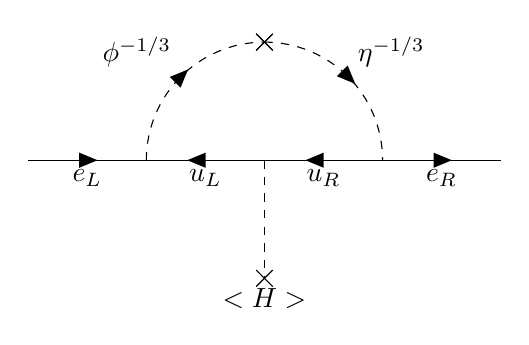
\begin{tikzpicture}
\begin{feynman}
\vertex (i);
\vertex [right = of i] (a);
\vertex [right = of a] (b);
\vertex [right = of b] (c);
\vertex [right = of c] (f);
\vertex [below = of b] (d) {$<H>$};
\vertex [above = of b] (u);

\diagram* {
(i) -- [fermion, edge label' = $e_L$] (a) -- [anti fermion, edge label' = $u_L$] (b),
(b) -- [anti fermion, edge label' = $u_R$] (c) -- [fermion, edge label' = $e_R$] (f),
(b) -- [scalar, insertion = 1] (d),
(a) -- [charged scalar, quarter left, edge label = $\phi^{-1/3}$] (u),
(u) -- [charged scalar, insertion = 0, quarter left, edge label = $\eta^{-1/3}$] (c),
};
\end{feynman}
\end{tikzpicture}
\caption{Diagram contributing to Dirac Charged Lepton Mass.}
\label{fig:Me}
\end{subfigure}
\caption{LeptoQuark mediated 1 loop Lepton Mass Diagrams.}
\end{figure}
\begin{equation*}
\feynmandiagram[horizontal=i to a]{
i -- [scalar, edge label = H] a,
a -- [anti fermion] f1[particle = $\overline{e^{-1}}$],
a -- [fermion] f2[particle = $e^{-1}$],
};
\quad \Gamma \sim m_e ?
\end{equation*}
\begin{equation*}
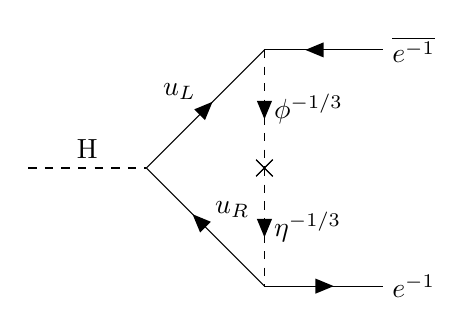
\begin{tikzpicture}
\begin{feynman}
\vertex (i);
\vertex [right = of i] (a);
\vertex [right = of a] (d);
\vertex [above = of d] (b);
\vertex [below = of d] (c);
\vertex [right = of b] (f1){$\overline{e^{-1}}$};
\vertex [right = of c] (f2){$e^{-1}$};

\diagram* {
(i) -- [scalar, edge label = H] (a),
(a) -- [fermion, edge label = $u_L$] (b),
(a) -- [anti fermion, edge label = $u_R$] (c),
(b) -- [anti fermion] (f1)[particle = $\overline{e^{-1}}$],
(c) -- [fermion] (f2)[particle = $e^{-1}$],
(b) -- [charged scalar, edge label = $\phi^{-1/3}$] (d),
(d) -- [charged scalar, insertion = 0, edge label = $\eta^{-1/3}$] (c),
};
\end{feynman}
\end{tikzpicture}
\quad \Gamma \sim m_e f \left(1+?\right)?
\end{equation*}
\section{Other tries}
\begin{centering}
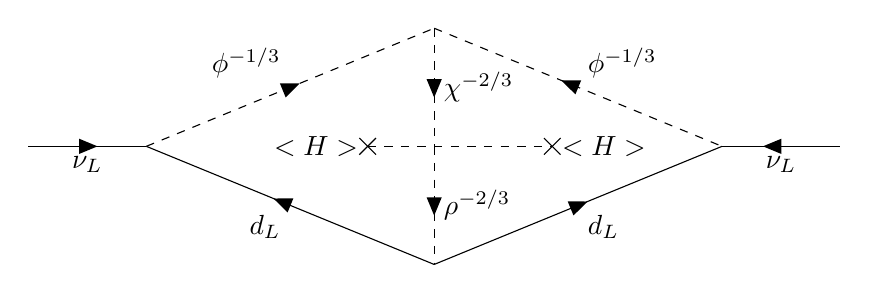
\begin{tikzpicture}
\begin{feynman}
\vertex (i);
\vertex [right = of i] (a);
\vertex [right = of a] (m1){$<H>$};
\vertex [right = of m1] (d);
\vertex [above = of d] (b);
\vertex [below = of d] (c);
\vertex [right = of d] (m2){$<H>$};
\vertex [right = of m2] (e);
\vertex [right = of e] (f);

\diagram* {
(i) -- [fermion, edge label' = $\nu_L$] (a),
(a) -- [anti fermion, edge label' = $d_L$] (c),
(c) -- [fermion, edge label' = $d_L$] (e),
(e) -- [anti fermion, edge label'=$\nu_L$] (f),
(a) -- [charged scalar, edge label=$\phi^{-1/3}$] (b),
(b) -- [anti charged scalar, edge label = $\phi^{-1/3}$] (e),
(b) -- [charged scalar, edge label = $\chi^{-2/3}$] (d),
(d) -- [charged scalar, edge label = $\rho^{-2/3}$] (c),
(m1) -- [scalar, insertion=0] (d),
(d) -- [scalar, insertion=1] (m2),
};
\end{feynman}
\end{tikzpicture}
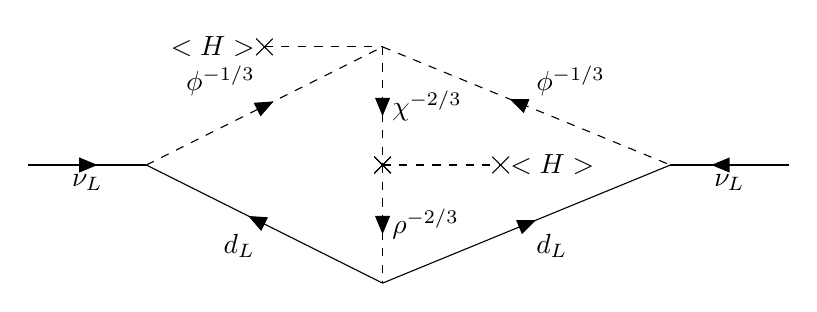
\begin{tikzpicture}
\begin{feynman}
\vertex (i);
\vertex [right = of i] (a);
\vertex [right = of a] (m1);
\vertex [right = of m1] (d);
\vertex [above = of d] (b);
\vertex [left = of b] (u1){$<H>$};
\vertex [below = of d] (c);
\vertex [right = of d] (m2){$<H>$};
\vertex [right = of m2] (e);
\vertex [right = of e] (f);

\diagram* {
(i) -- [fermion, edge label' = $\nu_L$] (a),
(a) -- [anti fermion, edge label' = $d_L$] (c),
(c) -- [fermion, edge label' = $d_L$] (e),
(e) -- [anti fermion, edge label'=$\nu_L$] (f),
(a) -- [charged scalar, edge label=$\phi^{-1/3}$] (b),
(b) -- [anti charged scalar, edge label = $\phi^{-1/3}$] (e),
(b) -- [charged scalar, edge label = $\chi^{-2/3}$] (d),
(d) -- [charged scalar, insertion=0, edge label = $\rho^{-2/3}$] (c),
(u1) -- [scalar, insertion=0] (b),
(d) -- [scalar, insertion=1] (m2),
};
\end{feynman}
\end{tikzpicture}
\end{centering}
\hrule
\section{1 loop, 1 LQ, $d_R$ mixing model}
\begin{figure}[h]
\centering
\begin{tikzpicture}
\begin{feynman}
\vertex (i);
\vertex [right = of i] (a);
\vertex [right = of a] (b);
\vertex [right = of b] (c);
\vertex [right = of c] (d);
\vertex [right = of d] (e);
\vertex [right = of e] (f);
\vertex [below = of b] (b1) {$<H>$};
\vertex [below = of c] (b2) {$<H>$};
\diagram*{
(i) -- [fermion, edge label' = $\nu_L$] (a) -- [fermion, edge label' = $d_L^c$] (b),
(b) -- [fermion, edge label' = $d_R^c$] (c) -- [fermion, edge label' = $a_L^c$] (d),
(d) -- [fermion, insertion=0, edge label' = $a_R^c$] (e) -- [fermion, edge label' = $\nu_L^c$] (f),
(a) -- [charged scalar, half left, edge label = $\phi^{-1/3}$] (e)[cross],
(b) -- [scalar, insertion = 1] (b1),
(c) -- [scalar, insertion = 1] (b2),
};
\end{feynman}
\end{tikzpicture}
\caption{Neutrino Mass Diagram through d quark mixing.}
\label{fig:daMnu}
\end{figure}
\begin{center}
\begin{tabular}[h]{|c|c|c|c|c|c|}
%\centering
\hline
Particle & SU(3)$_c$ & SU(2)$_L$ & U(1)$_Y$ & S & Flavour \\ \hline
Q & 3 & 2 & 1/6 &  & 3 \\
d$_R^c$ & 3$^*$ & 1 & +1/3 &  & 3 \\
u$_R^c$ & 3$^*$ & 1 & -2/3 &  & 3 \\
L & 1 & 2 & -1/2 &  & 3 \\
e$_R^c$ & 1 & 1 & +1 &  & 3 \\
A$_{R,L}$ & 3 & 2 & -5/6 &  & 3 \\
H & 1 & 2 & 1/2 &  & 1 \\
$\phi$ & 3 & 1 & -1/3 &  & 1 \\ \hline
\end{tabular}
\end{center}
\begin{align*}
\mathcal{L}_{new,4D}^Y\,&\subset \, y_1\, \underbrace{\overline{Q_L^c} L}_{\mathclap{\left(\overline{d_L^c} \nu_L - \overline{u_L^c} e_L\right)}} \phi^* + y_2\, \overline{u_R^c} e_R \phi^* + y_3\, \overline{A_R} L \phi + y_{\epsilon} \overline{d_R} A_L H + h.c. \\
\mathcal{L}_{3D}\,&\subset\,\mathcal{M}_A \overline{A} A \\
V(H,\phi)\,&=\, -m_1^2 \left|H\right|^2 + \frac{\lambda_1}{4} \left|H\right|^4 + m_2^2 \left|\phi\right|^2 + \frac{\lambda_2}{4} \left|\phi\right|^4 + \lambda_3 \left(H^{\dagger}H\right)\left|\phi\right|^2
\end{align*}
\end{document}